\section{Results}\label{sr.res}
The search yielded 1384 publications,
of which 94 studies were included (Figure~\ref{fig:sr.prisma}).
These studies (\srds{A})
applied non-linear compartmental modelling to simulate ART scale-up in SSA,
of which 40 reported infections averted/incidence reduction
due to population-wide ART scale-up without combination intervention,
relative to a base-case reflecting status quo (\srds{B}).
\begin{figure}
  \centering
  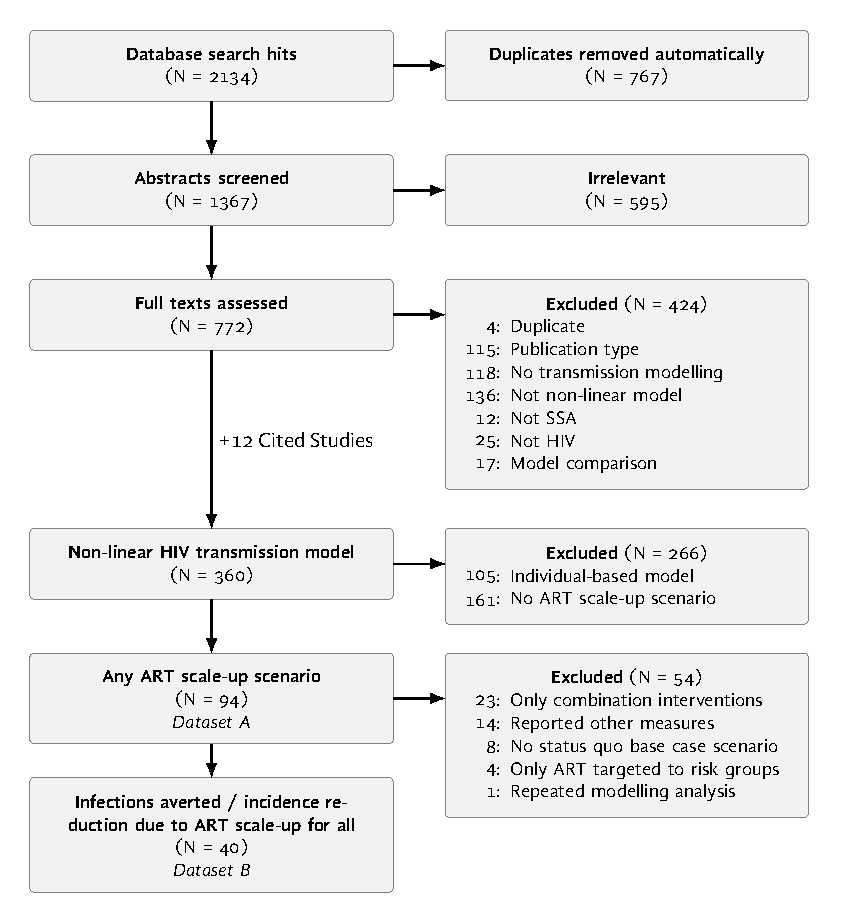
\includegraphics[scale=1]{sr.prisma}
  \caption{PRISMA flowchart of study identification}
  \label{fig:sr.prisma}
\end{figure}
%===================================================================================================
\subsection{Epidemic Context}\label{sr.res.context}
Table~\ref{tab:sr.summary} summarizes key features of contexts within SSA
where the prevention impacts of ART have been modelled.
61 studies modelled HIV transmission at the national level;
studies also explored
regional (1), sub-national (16), and city-level (16) epidemic scales.
South Africa was the most common country simulated (52 studies);
Figure~\ref{fig:sr.map} illustrates the number of studies by country.
East Africa was the most represented SSA region, being simulated in 77 studies,
followed by Southern (72), West (28), and Central Africa (13).
\begin{table}
  \centering
  \caption{Summary of epidemic contexts within Sub-Saharan Africa where
    the prevention impacts of ART have been modelled}
  \label{tab:sr.summary}
  \begin{tabular}{llr}
\toprule
\multicolumn{2}{l}{Study Characteristic} & Studies \\
\midrule
Geographic scale & Regional              & 1  \\
                 & National              & 61 \\
                 & Sub-national          & 16 \\
                 & City                  & 16 \\
\midrule
Modelled         & South Africa          & 52 \\
countries\tn{a}  & Kenya                 & 22 \\
                 & Zambia                & 10 \\
                 & Other                 & 29 \\
\midrule
HIV prevalence   & Low ($<$1\%)          &  0 \\
                 & Mid (1-10\%)          & 23 \\
                 & High ($>$10\%)        & 41 \\
                 & Unclear/Varies        & 30 \\
\midrule
Incidence trend  & Decreasing            & 10 \\
at scenario      & Dec-to-stable         & 24 \\
divergence       & Stable                & 11 \\
                 & Inc-to-stable         &  1 \\
                 & Increasing            &  2 \\
                 & Unclear/Varies        & 46 \\
\midrule
Key populations  & FSW\tn{b}             & 39 \\
included         & Clients\tn{c}         & 31 \\
                 & MSM                   & 28 \\
                 & Transgender           &  0 \\
                 & PWID                  & 11 \\
                 & Prisoners             &  2 \\
\bottomrule
\end{tabular}
\floatfoot{
  Total studies: 94.
  FSW: female sex workers;
  Clients: clients of sex workers;
  MSM: men who have sex with men;
  PWID: people who inject drugs;
  \tnt[a]{does not sum to 94 as some studies modelled multiple countries};
  \tnt[b]{groups described as FSW,
    not considering the epidemiological definitions given in Appendix~\ref{app.sr.defs.kp}};
  \tnt[c]{likewise for clients, and excluding studies where clients were modelled
    as a proportion of another risk group}.
}
\end{table}
\par
ART prevention impacts were most often modelled in
high-prevalence ({$>$\,10\%}) epidemics (41 studies) and
medium-prevalence ({1--10\%}) epidemics (23) (Figure~\ref{fig:sr.dist.api.prev}).
No studies reported overall HIV prevalence of {$<$\,1\%} at time of intervention,
although for 30 studies, HIV prevalence was
not reported or varied across simulated contexts/scenarios.
The median [min, (IQR), max] year of intervention was 2014 [1990, (2010, 2015), 2040]; at which time
HIV prevalence (\%) was 15 [2, (6, 19), 32] (Figure~\ref{fig:sr.dist.api.prev}); and
incidence (per 1000 person-years) was 14 [1, (9, 20), 50] (Figure~\ref{fig:sr.dist.api.inc}).
Most reported incidence trends were decreasing or stable
(45 of 48 reporting, Figure~\ref{fig:sr.dist.api.phase}).
%---------------------------------------------------------------------------------------------------
\subsubsection{Key Populations}\label{sr.res.context.kp}
FSW were explicitly modelled in 39 studies.
Among these (of studies where it was possible to evaluate):
21 (of 25) were {$<$\,5\%} of the female population;
14 (of 24) were {$<$\,1/3} the size of the client population; and
15 (of 22) had {$>$\,50$\times$} partners per year versus
the lowest sexually active female activity group.
Clients of FSW were modelled as a unique group in 31 studies,
among which 8 (of 17 reporting) were {$>$\,3$\times$} the size of the FSW population.
In another 8 studies, clients were defined as a proportion of another group,
among which 6 (of 7) were {$>$\,3$\times$} the FSW population size.
Studies explicitly modelled men who have sex with men (MSM) in 28 studies;
transgender in 0; people who inject drugs (PWID) in 11; and prisoners in 2.
%===================================================================================================
\subsection{Heterogeneity Factors}\label{sr.res.f}
%---------------------------------------------------------------------------------------------------
\subsubsection{Biological Effects}\label{sr.res.f.bio}
The median [min, (IQR), max] number of states used to represent HIV disease
(ignoring treatment-related stratifications) was 5 [1, (3, 6), 25] (Figure~\ref{fig:sr.dist.hiv.n}),
and 2 studies represented HIV along a continuous dimension using partial differential equations.
States of increased infectiousness associated with acute infection and late-stage disease
were simulated in 68 and 74 studies, respectively.
\par
The relative risk of HIV transmission on ART was 0.08 [0, (0.04, 0.13), 0.3]
(Figure~\ref{fig:sr.dist.art.rbeta}),
representing an average ``on-treatment'' state in 78 studies,
versus a ``virally suppressed'' state in 15.
Treatment failure due to drug resistance was simulated in 24 studies, including:
23 where individuals experiencing treatment failure were tracked separately from ART-naive;
and 1 where such individuals transitioned back to a generic ``off-treatment'' state.
Another 6 studies included a similar transition
that was not identified as treatment failure versus ART cessation.
Transmissible drug resistance was simulated in 9 studies.
%---------------------------------------------------------------------------------------------------
\subsubsection{Behavioural Effects}\label{sr.res.f.behav}
Reduced sexual activity during late-stage HIV was simulated in 25 studies,
including at least one state with:
complete cessastion of sexual activity (14);
reduced rate/number of partnerships (9); and/or
reduced rate/number of sex acts per partnership (6).
\par
Separate health states representing diagnosed HIV before treatment,
and on-treatment before viral suppression were simulated in
30 and 17 studies, respectively.
22 studies modelled behaviour changes following awareness of HIV+ status, including:
increased condom use (12);
fewer partners per year (4);
fewer sex acts per partnership (3);
serosorting (1); and/or
a generic reduction in transmission probability (8).
\par
ART cessation was simulated in 35 studies, including:
16 where individuals no longer on ART were tracked separately from ART-naive; and
19 where such individuals transitioned back to a generic ``off-treatment'' state.
Another 6 studies included a similar transition
that was not identified as treatment failure versus ART cessation.
%---------------------------------------------------------------------------------------------------
\subsubsection{Network Effects}\label{sr.res.f.net}
Populations were stratified by activity (different rates and/or types of partnerships formed)
in 59 studies, and by sex/gender in 64.
The number of groups defined by sex/gender and/or activity was 6 [1, (2, 9), 19] (Figure~\ref{fig:sr.dist.act.n});
and by activity alone (maximum number of groups among:
women who have sex with men, men who have sex with women,
MSM, or overall if sex/gender was not considered) was 3 [1, (1, 3), 18].
The highest activity groups for females and males (possibly including FSW/clients) comprised
2 [$<$\,1, (2, 4), 23] and 9 [$<$\,1, (2, 14), 35]\% of female and male populations, respectively
(Figures~\ref{fig:sr.dist.act.HRW.p} and \ref{fig:sr.dist.act.HRM.p}).
\par
Turnover between activity groups and/or key populations was considered in 28 studies,
of which 9 considered turnover of only one specific high-activity group or key population.
Another 7 studies simulated movement only from lower to higher activity groups
to re-balance group sizes against disproportionate HIV mortality.
\par
Among 59 studies with activity groups, sexual mixing was modelled as
assortative in 57 and proportionate in 2.
Partnerships had equal probability of transmission in 39 studies,
including all studies without activity groups.
Partnerships were defined by the activity groups involved in 44 studies,
among which transmission was usually
lower in high-with-high activity partnerships than in low-with-low, due to
fewer sex acts (31) and/or increased condom use (23).
Transmission risk in high-with-low activity partnerships was defined by the:
susceptible partner (9);
lower activity partner (11);
higher activity partner (3); or
both partners' activity groups (15); yielding
indeterminate, higher, lower, or intermediate per-partnership transmission risk, respectively.
Partnerships were defined based on overlapping types, such that
different partnership types could be formed between the same two activity groups in 11 studies.
All overlapping partnership types had differential total sex acts and condom use.
\par
Age groups were simulated in 32 studies, among which,
the number of age groups was 10 [2, (4, 34), 91] (Figure~\ref{fig:sr.dist.age.n}),
and 2 studies simulated age along a continuous dimension.
Sexual mixing between age groups was assumed to be assortative
either with (23) or without (3) average age differences between men and women;
or proportionate (6).
Differential risk behaviour by age was modelled in 29 studies.
%---------------------------------------------------------------------------------------------------
\subsubsection{Cascade Effects}\label{sr.res.f.cascade}
Differential transition rates along the ART cascade were considered in
21 studies, including differences between
genders in 15; age groups in 7; and key populations in 12.
Another 2 studies did not simulate differential cascade transitions,
but justified the decision using context-specific data.
Differences between genders included rates of
HIV diagnosis (11); ART initiation (6); and ART cessation (1),
with cascade engagement higher among women,
in most cases attributed to antenatal services.
Differences between age groups also affected
rates of diagnosis (6); ART initiation (1); but not ART cessation (0).
Among key populations, \emph{lower} rates of
diagnosis, ART initiation, and retention were simulated in 0, 2, and 4
studies respectively, while \emph{higher} rates were simulated in 8, 2, and 1.
%===================================================================================================
\subsection{ART Prevention Impact}\label{sr.res.api}
\srds{B} comprised 40 studies, including 125 scenarios of ART scale-up.
Relative incidence reduction (IR) with ART scale-up as compared to status quo
was reported in 23 studies (61 scenarios);
proportion of cumulative infections averted (CIA) due to ART scale-up
in 24 (75); and 7 (11) reported both.
Some scenarios included multiple time horizons.
\begin{table}
  \centering
  \caption{Projected ART prevention impacts,
    stratified by factors of risk heterogeneity and contexts}
  \label{tab:sr.api}
  \def\baselinestretch{1.0}\footnotesize
\newcommand{\xpos}[1]{\ifnum#1<9\relax\d#1\else#1\fi}
\newcommand{\xneg}[1]{%
  \ifnum#1<-99\relax#1\else
  \ifnum#1<-9\relax\d#1\else
  \ifnum#1<0\relax\d\d#1\else
  \ifnum#1<10\relax\d\d\m#1\else
  \ifnum#1<100\relax\d\m#1\else\m#1%
  \fi\fi\fi\fi\fi}
\newcommand{\pci}[2]{(\,\xpos{#1},\,\xpos{#2}\,)}
\newcommand{\nci}[2]{(\,\xneg{#1},\,\xneg{#2}\,)}
\setlength{\tabcolsep}{.5em}
\centerline{
\begin{tabular}{ll|rrcrc|rrcrc}
  \toprule
  & & \multicolumn{5}{c}{Incidence Reduction (\%)}
    & \multicolumn{5}{c}{Cumulative Infections Averted (\%)} \\
  \cmidrule(rl){3-7}\cmidrule(rl){8-12}
  Factor               & Level            & N\tn{a} & \multicolumn{2}{c}{Median (IQR)} & \multicolumn{2}{c}{Effect (95\% CI)\tn{b}} 
                                          & N\tn{a} & \multicolumn{2}{c}{Median (IQR)} & \multicolumn{2}{c}{Effect (95\% CI)\tn{b}} \\
  \midrule
  Risk Stratif. \&     & None             &  98 &  19 & \pci{7}{44}   & \REF &               &  45 & 29 & \pci{18}{47} & \REF &                 \\
  Cascade Diff.        & Activity (No KP) &  22 &  35 & \pci{22}{46}  &    4 & \nci{-14}{22} &  39 &  6 & \pci{3}{22}  &   24 & \nci{12}{36}    \\
                       & + KP (Same)      &   5 &  41 & \pci{6}{50}   &   72 & \nci{-31}{175}&   8 & 10 & \pci{3}{21}  &   20 & \nci{11}{28}    \\
                       & + KP (Priority)  &   1 &  85 & \pci{85}{85}  &  136 & \nci{73}{199} &  23 & 21 & \pci{11}{41} &  131 & \nci{97}{166}   \\[1ex]
  Activity Turnover    & No               & 117 &  26 & \pci{8}{45}   & \REF &               &  87 & 20 & \pci{5}{35}  & \REF &                 \\
                       & Yes              &   9 &  22 & \pci{21}{50}  &  -82 &\nci{-153}{-11}&  28 & 18 & \pci{7}{38}  &  -86 & \nci{-103}{-70} \\[1ex]
  Sex/Gender Stratif.  & No               &  97 &  21 & \pci{7}{44}   & \REF &               &  39 & 29 & \pci{18}{44} & \REF &                 \\
  \& Cascade Diff.     & Yes (Same)       &  22 &  41 & \pci{30}{53}  &   -4 & \nci{-32}{23} &  48 &  8 & \pci{3}{24}  &  -49 & \nci{-62}{-36}  \\
                       & Yes (Men Low)    &   7 &  21 & \pci{2}{22}   &    5 & \nci{-41}{50} &  28 & 16 & \pci{4}{35}  & -125 & \nci{-143}{-108}\\[1ex]
  Partnership Types    & Generic          & 107 &  21 & \pci{8}{44}   & \REF &               &  48 & 28 & \pci{15}{42} & \REF &                 \\
                       & By Groups        &  16 &  33 & \pci{22}{52}  &  -22 & \nci{-53}{9}  &  66 & 11 & \pci{3}{28}  &   34 & \nci{20}{49}    \\
                       & Overlapping      &   3 &  50 & \pci{45}{62}  &    8 & \nci{-52}{69} &   1 & 58 & \pci{58}{58} &   -9 & \nci{-60}{43}   \\ \midrule
  Time Horizon         & 0-10             &  36 &  17 & \pci{7}{35}   & \REF &               &  40 & 14 & \pci{3}{26}  & \REF &                 \\
  (years)              & 11-20            &  63 &  20 & \pci{8}{42}   &    3 & \nci{-3}{9}   &  60 & 22 & \pci{8}{38}  &    9 & \nci{2}{17}     \\
                       & 21-30            &  15 &  47 & \pci{39}{65}  &    3 & \nci{-7}{13}  &  11 & 23 & \pci{7}{47}  &   12 & \nci{6}{19}     \\
                       & 31+              &  12 &  46 & \pci{24}{57}  &   12 & \nci{5}{20}   &   4 & 34 & \pci{29}{40} &    5 & \nci{1}{8}      \\[1ex]
  HIV Prevalence       & 11+              & 112 &  22 & \pci{8}{44}   & \REF &               &  75 & 18 & \pci{4}{35}  & \REF &                 \\
  (\%)                 & 1-10             &  14 &  43 & \pci{36}{49}  &   -9 & \nci{-49}{31} &  39 & 26 & \pci{11}{36} &   -9 & \nci{-20}{2}    \\
                       & 0-1              &   0 & --- &      ---      &      &               &   1 & 49 & \pci{49}{49} &   -3 & \nci{-30}{24}   \\[1ex]
  HIV Incidence        & Increasing       &   2 &  40 & \pci{38}{43}  &      &               &   5 & 32 & \pci{29}{41} &      &                 \\
  Trend\tn{c}          & Inc-to-stable    &   1 &  97 & \pci{97}{97}  &      &               &   1 & 68 & \pci{68}{68} &      &                 \\
                       & Stable           &  17 &  21 & \pci{20}{29}  &      &               &  24 &  4 & \pci{2}{7}   &      &                 \\
                       & Dec-to-stable    &  81 &  15 & \pci{6}{43}   &      &               &  11 &  1 & \pci{-8}{28} &      &                 \\
                       & Decreasing       &   1 &  57 & \pci{57}{57}  &      &               &  13 & 29 & \pci{19}{38} &      &                 \\ \midrule
  RR Transmission      & 0.0-0.039        &  11 &  22 & \pci{14}{35}  & \REF &               &  44 &  6 & \pci{2}{27}  & \REF &                 \\
  on ART               & 0.04-0.099       &  42 &  49 & \pci{34}{67}  &   55 & \nci{22}{89}  &  60 & 27 & \pci{15}{38} &  -41 & \nci{-54}{-29}  \\
                       & 0.1+             &  73 &  12 & \pci{5}{30}   &    9 & \nci{-31}{48} &  11 & 19 & \pci{1}{33}  &  -20 & \nci{-26}{-13}  \\[1ex]
  CD4 Threshold for    & Symptomatic      &   3 &  38 & \pci{37}{41}  &   47 & \nci{25}{68}  &  24 &  4 & \pci{2}{7}   &  -30 & \nci{-46}{-15}  \\
  ART Initiation       & 200              &   3 &  28 & \pci{26}{32}  & \REF &               &   4 & 28 & \pci{24}{30} & \REF &                 \\
                       & 350              &  10 &  29 & \pci{22}{38}  &   15 & \nci{3}{28}   &  18 & 18 & \pci{13}{27} &    3 & \nci{-2}{7}     \\
                       & 500              &  15 &  29 & \pci{16}{43}  &   27 & \nci{8}{45}   &  13 & 29 & \pci{23}{35} &   17 & \nci{10}{24}    \\
                       & Any              &  41 &  56 & \pci{22}{75}  &   30 & \nci{14}{47}  &  22 & 51 & \pci{28}{62} &   42 & \nci{37}{48}    \\
                       & Mixed            &  54 &  10 & \pci{5}{31}   &    1 & \nci{-31}{32} &  34 & 16 & \pci{5}{37}  &   63 & \nci{54}{72}    \\[1ex]
  ART Coverage         & 0-59             &   3 &  28 & \pci{26}{31}  &      &               &  11 & 30 & \pci{13}{43} &      &                 \\
  Target (\%)\tn{c}    & 60-84            &  13 &  29 & \pci{21}{41}  &      &               &  22 & 22 & \pci{8}{39}  &      &                 \\
                       & 85+              &  13 &  46 & \pci{36}{66}  &      &               &  21 & 36 & \pci{26}{43} &      &                 \\ \midrule
  Acute Infection      & No               &  35 &  22 & \pci{10}{57}  & \REF &               &  15 & 38 & \pci{24}{50} & \REF &                 \\
                       & Yes              &  91 &  26 & \pci{9}{44}   &   52 & \nci{13}{91}  & 100 & 16 & \pci{5}{32}  &   51 & \nci{36}{66}    \\[1ex]
  Late-Stage Infection & No               &  38 &  39 & \pci{13}{56}  & \REF &               &  12 & 36 & \pci{20}{48} & \REF &                 \\
                       & Yes              &  88 &  22 & \pci{8}{43}   &  -23 & \nci{-37}{-8} & 103 & 18 & \pci{5}{34}  &  -37 & \nci{-65}{-9}   \\[1ex]
  Trans. Drug Resist.  & No               & 114 &  21 & \pci{7}{43}   & \REF &               & 102 & 18 & \pci{5}{36}  & \REF &                 \\
                       & Yes              &  12 &  72 & \pci{39}{85}  &   -4 & \nci{-46}{39} &  13 & 26 & \pci{20}{30} &   -3 & \nci{-8}{3}     \\ \midrule
  HIV Morbidity        & No               & 102 &  21 & \pci{7}{45}   & \REF &               &  73 & 27 & \pci{13}{42} & \REF &                 \\
                       & Any              &  24 &  34 & \pci{22}{46}  &   35 & \nci{16}{54}  &  42 &  6 & \pci{3}{23}  &  -20 & \nci{-26}{-14}  \\[1ex]
  HTC Behav. Change    & No               & 112 &  21 & \pci{7}{45}   & \REF &               &  81 & 23 & \pci{11}{38} & \REF &                 \\
                       & Any              &  14 &  41 & \pci{29}{49}  &  -39 & \nci{-73}{-4} &  34 &  6 & \pci{3}{22}  &  -13 & \nci{-18}{-7}   \\
  \bottomrule
\end{tabular}}
\floatfoot{
  \tnt[a]{N: number of unique scenarios and time horizons;
    sums across factor levels may be less than 126 and 115 due to missing variables.}
  \tnt[b]{Effect estimates from linear multivariable regression
    with generalized estimating equations \cite{Hojsgaard2006};
    effects are illustrated in Figure~C.20.}
  \tnt[c]{Omitted from regression model due to missing data.}
  RR: relative risk;
  HTC: HIV testing and counselling;
  KP: key populations.
  priority: modelled ART cascade transitions were faster in KP vs overall due to prioritized programs;
  same: cascade transitions were assumed the same in KP as overall.
  Factor definitions are given in Appendix~B.
}
\end{table}
\begin{figure}[h]
  \centering
  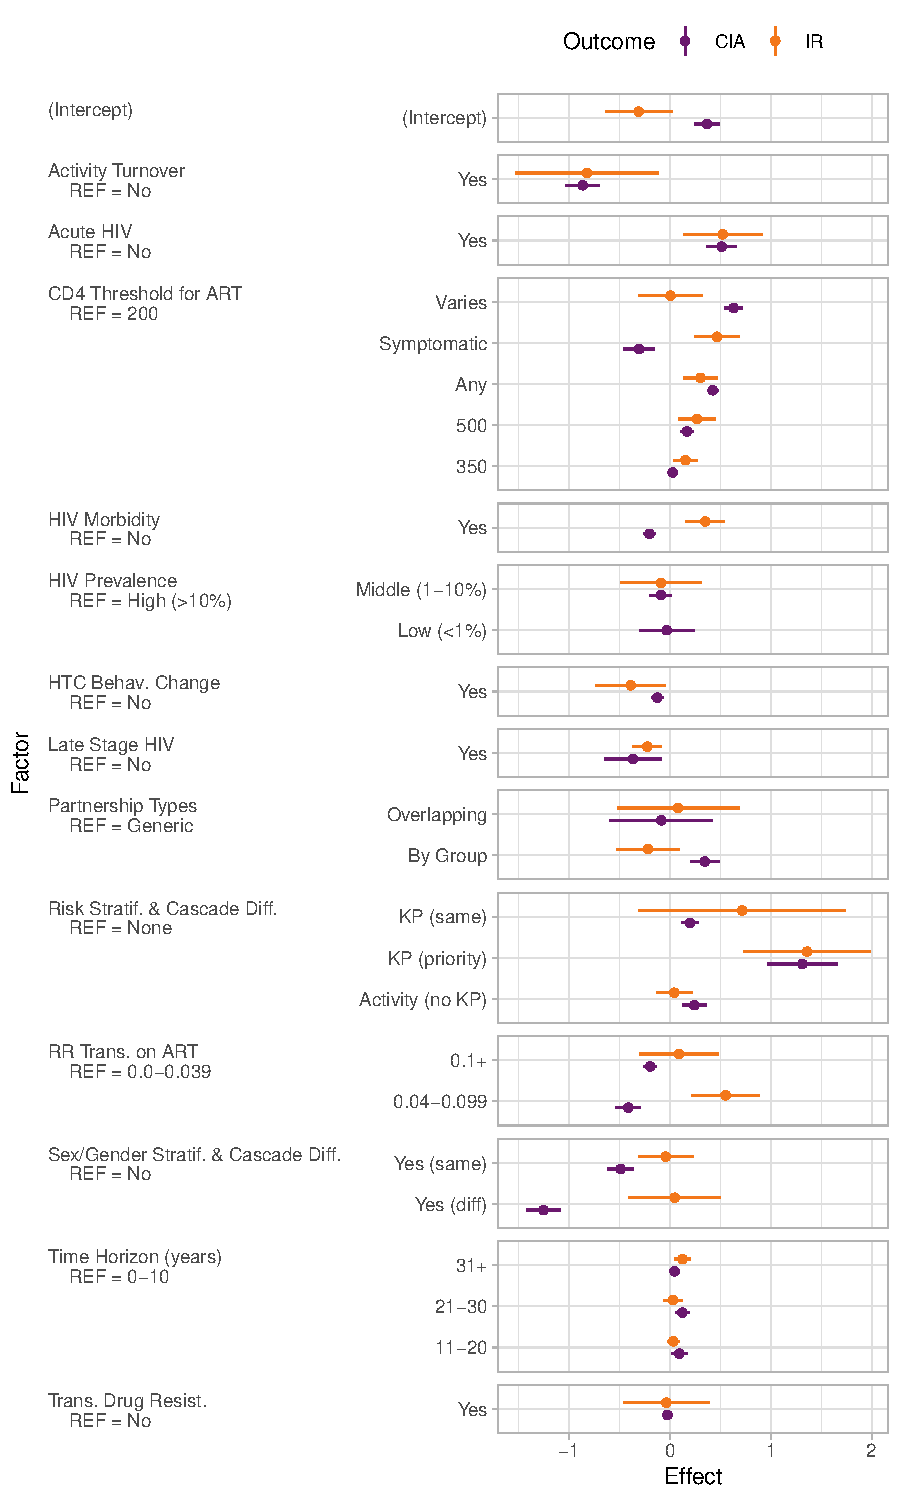
\includegraphics[height=\dimexpr\textheight-8\baselineskip]{sr.effects}
  \caption{Effect estimates for factors of heterogeneity on
    incidence reduction (\%, IR) and cumulative infections averted (\%, CHI)
    from linear multivariate regression with generalized estimating equations.}
  \label{fig:sr.effects}
  \floatfoot{
    Numerical results given in Table~\ref{tab:sr.api}.
    RR: relative risk;
    HTC: HIV testing and counselling;
    KP: key populations.
    priority: modelled ART cascade transitions were faster in KP vs overall due to prioritized programs;
    same: cascade transitions were assumed the same in KP as overall.
    Factor definitions are given in Appendix~\ref{app.sr.defs}.}
\end{figure}
Table~\ref{tab:sr.api} summarizes projected ART prevention impacts (IR, CIA),
stratified by heterogeneity and contextual factors,
plus adjusted effect estimates for each factor from multivariate analysis.
Figure~\ref{fig:sr.api} illustrates
unadjusted impacts stratified by factor levels, while
Figures~\ref{fig:sr.effects} illustrates adjusted effect estimates.
Compared to models with homogeneous risk,
including risk heterogeneity via static activity groups but without key populations
was associated with slightly higher impacts---adjusted effect (95\% CI):
4~($-$14,~22)\% IR, 24~(12,~36)\% CIA.
Including key population(s) and assuming similar ART cascade across groups
was also associated with higher impact:
72~($-$31,~175)\% IR, 20~(11,~28)\% CIA.
However, including turnover of one/more higher risk group(s)
was associated with smaller ART prevention impacts:
$-$82~($-$153,~$-$11)\% IR, $-$86~($-$103,~$-$70)\% CIA.
Taken together, models that captured heterogenetiy in risk across
activity groups and/or key population(s) with turnover
were associated with reduced ART prevention impacts.
\par
After including risk heterogeneity,
further capturing differential ART cascade across activity groups or key populations
was associated with differences in projected ART prevention impacts.
Models stratified by sex/gender, and those that captured lower ART cascade among men
were associated with a smaller CIA:
$-$49~($-$62,~$-$36)\% and $-$125~($-$143,~$-$108)\%, respectively;
although similar effects were not observed for IR:
$-$4~($-$32,~23)\% and 5~($-$41,~50)\%.
Where key populations were expliciltly modelled,
including ART cascade prioritized to any key population(s)
was associated with increased impact, enough to overcome reductions due to turnover:
136~(73,~199)\% IR, 131~(97,~166)\% CIA.
No studies in \srds{B} examined lower ART cascade among key population(s).
